\subsection{Corridas realizadas}

La corrida oficial se hizo el 22 de noviembre de 2026 en una sola máquina: Windows~11, un procesador Intel Core i7-14700 con 28 hilos, 63,7~GB de RAM y CPython~3.13.15, con \texttt{grpcio}~1.85.3 y \texttt{protobuf}~7.36.2. El script \texttt{correr\_experimento.py} ejecutó las 78 corridas del plan en unos 88~segundos y todas terminaron con estado \texttt{ok}. De ellas, 48 son de latencia (dos escenarios, dos tamaños, la corrida de calentamiento y cinco repeticiones, con cada mecanismo) y 30 son de intercambios de Lamport (2, 3 y 4 nodos, cinco repeticiones con cada mecanismo).

Los CSV crudos están sin editar en \texttt{data/}, junto con su archivo \texttt{SHA256SUMS}. Todas las tablas y figuras de esta sección salen de \texttt{analysis/analizar.py}, que las genera a partir de esos archivos; ninguna se armó a mano. Antes de calcular, el script descarta la repetición de calentamiento \texttt{r0} de cada condición (1600 envíos) y las dos corridas de prueba del 21 de noviembre, que no siguen el protocolo. Quedan 8000 envíos, 4000 por mecanismo.

\subsection{Latencia y mensajes por segundo}

\begin{table}[htbp]
  \centering
  \caption{Latencia de ida y vuelta (ms) y mensajes por segundo, sin la corrida de calentamiento}
  \label{tab:resumen}
  \resizebox{\textwidth}{!}{% Generado por analysis/analizar.py. No editar a mano.
% Latencias en ms (RTT). Msg/s: media de las repeticiones.
\begin{tabular}{llrrrrrrrrr}
\toprule
Mecanismo & Clientes & Tamaño & Rep. & Envíos & Media & Mediana & Desv. est. & P95 & Msg/s & IC 95\,\% msg/s \\
\midrule
Sockets TCP + JSON & 1 cliente & 100 B & 5 & 500 & 0.161 & 0.045 & 1.421 & 0.103 & 7747.0 & $\pm$4889.1 \\
gRPC + Protobuf & 1 cliente & 100 B & 5 & 500 & 0.358 & 0.291 & 0.616 & 0.365 & 2639.8 & $\pm$88.1 \\
Sockets TCP + JSON & 1 cliente & 10 KB & 5 & 500 & 0.157 & 0.072 & 1.117 & 0.152 & 6991.9 & $\pm$2843.9 \\
gRPC + Protobuf & 1 cliente & 10 KB & 5 & 500 & 0.371 & 0.303 & 0.598 & 0.408 & 2557.0 & $\pm$61.9 \\
Sockets TCP + JSON & 3 clientes & 100 B & 5 & 1500 & 0.152 & 0.056 & 1.171 & 0.132 & 12306.1 & $\pm$4831.0 \\
gRPC + Protobuf & 3 clientes & 100 B & 5 & 1500 & 0.426 & 0.366 & 0.579 & 0.499 & 5635.9 & $\pm$782.8 \\
Sockets TCP + JSON & 3 clientes & 10 KB & 5 & 1500 & 0.183 & 0.086 & 1.198 & 0.170 & 10992.8 & $\pm$3992.1 \\
gRPC + Protobuf & 3 clientes & 10 KB & 5 & 1500 & 0.461 & 0.396 & 0.599 & 0.531 & 5790.6 & $\pm$577.8 \\
\bottomrule
\end{tabular}
}
\end{table}

En la Tabla~\ref{tab:resumen}, la media, la mediana, la desviación estándar y el percentil~95 se calculan con todos los envíos de cada condición. Los mensajes por segundo son la media de las cinco repeticiones, con su intervalo de confianza del 95\,\% (t de Student con cuatro grados de libertad).

Con un cliente y 100~bytes, la mediana de sockets fue 0,045~ms y la de gRPC 0,291~ms, unas 6,5 veces más. La diferencia aparece igual en cada repetición: las medianas de sockets quedaron entre 0,043 y 0,046~ms y las de gRPC entre 0,288 y 0,295~ms. El percentil~95 fue de 0,103~ms con sockets y de 0,365~ms con gRPC.

Con 10~KB subieron las dos latencias, pero no en la misma proporción. La mediana de sockets pasó de 0,045 a 0,072~ms, un 60\,\% más, y la de gRPC de 0,291 a 0,304~ms, apenas un 4\,\% más. En milisegundos la distancia entre los dos mecanismos casi no cambió: unos 0,25~ms con 100~bytes y 0,23~ms con 10~KB.

Con tres clientes enviando a la vez al nodo~A, las medianas con 100~bytes fueron de 0,056~ms con sockets y de 0,366~ms con gRPC. Frente a un cliente, las dos subieron en proporción parecida: un 24\,\% sockets y un 26\,\% gRPC. Donde sí hay diferencia es en los mensajes por segundo de los tres clientes juntos. gRPC pasó de 2640 a 5636, es decir, algo más del doble, mientras que sockets pasó de 7747 a 12\,306, un 59\,\% más.

\begin{figure}[htbp]
  \centering
  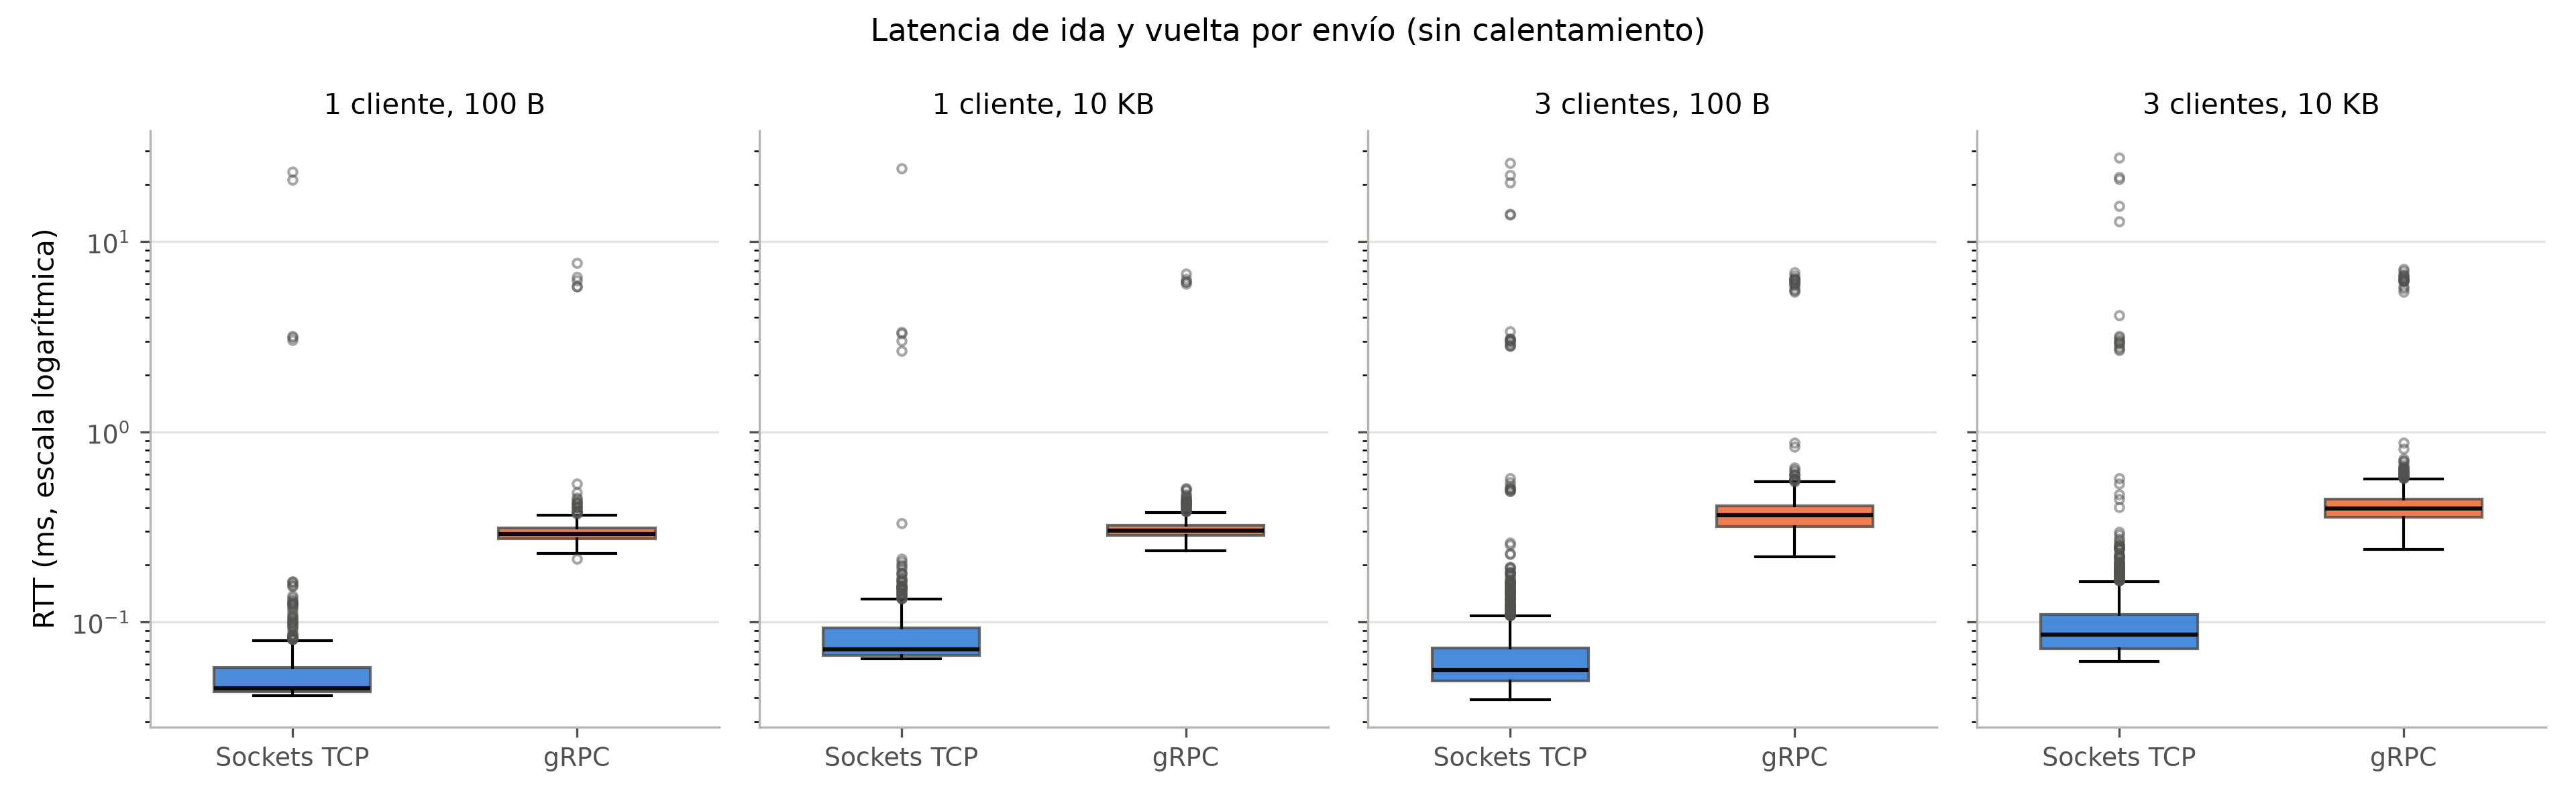
\includegraphics[width=\textwidth]{boxplot}
  \caption{Latencia de ida y vuelta de cada envío por condición, en escala logarítmica}
  \label{fig:boxplot}
\end{figure}

La Figura~\ref{fig:boxplot} muestra cómo se reparten los envíos. gRPC tiene una distribución estrecha, y su envío más lento tardó 7,8~ms. Sockets tiene la mediana más baja en las cuatro condiciones, pero 13 de sus 4000 envíos pasaron de 10~ms, con un máximo de 27,6~ms. Cuando uno de esos envíos cae en una repetición, alarga su duración, y por eso los mensajes por segundo de sockets cambian tanto de una repetición a otra: con un cliente y 100~bytes van de 3316 a 10\,850. Esa es la razón de que sus intervalos de confianza sean tan anchos en la Figura~\ref{fig:barras}. La mediana casi no se mueve con estos casos aislados.

\begin{figure}[htbp]
  \centering
  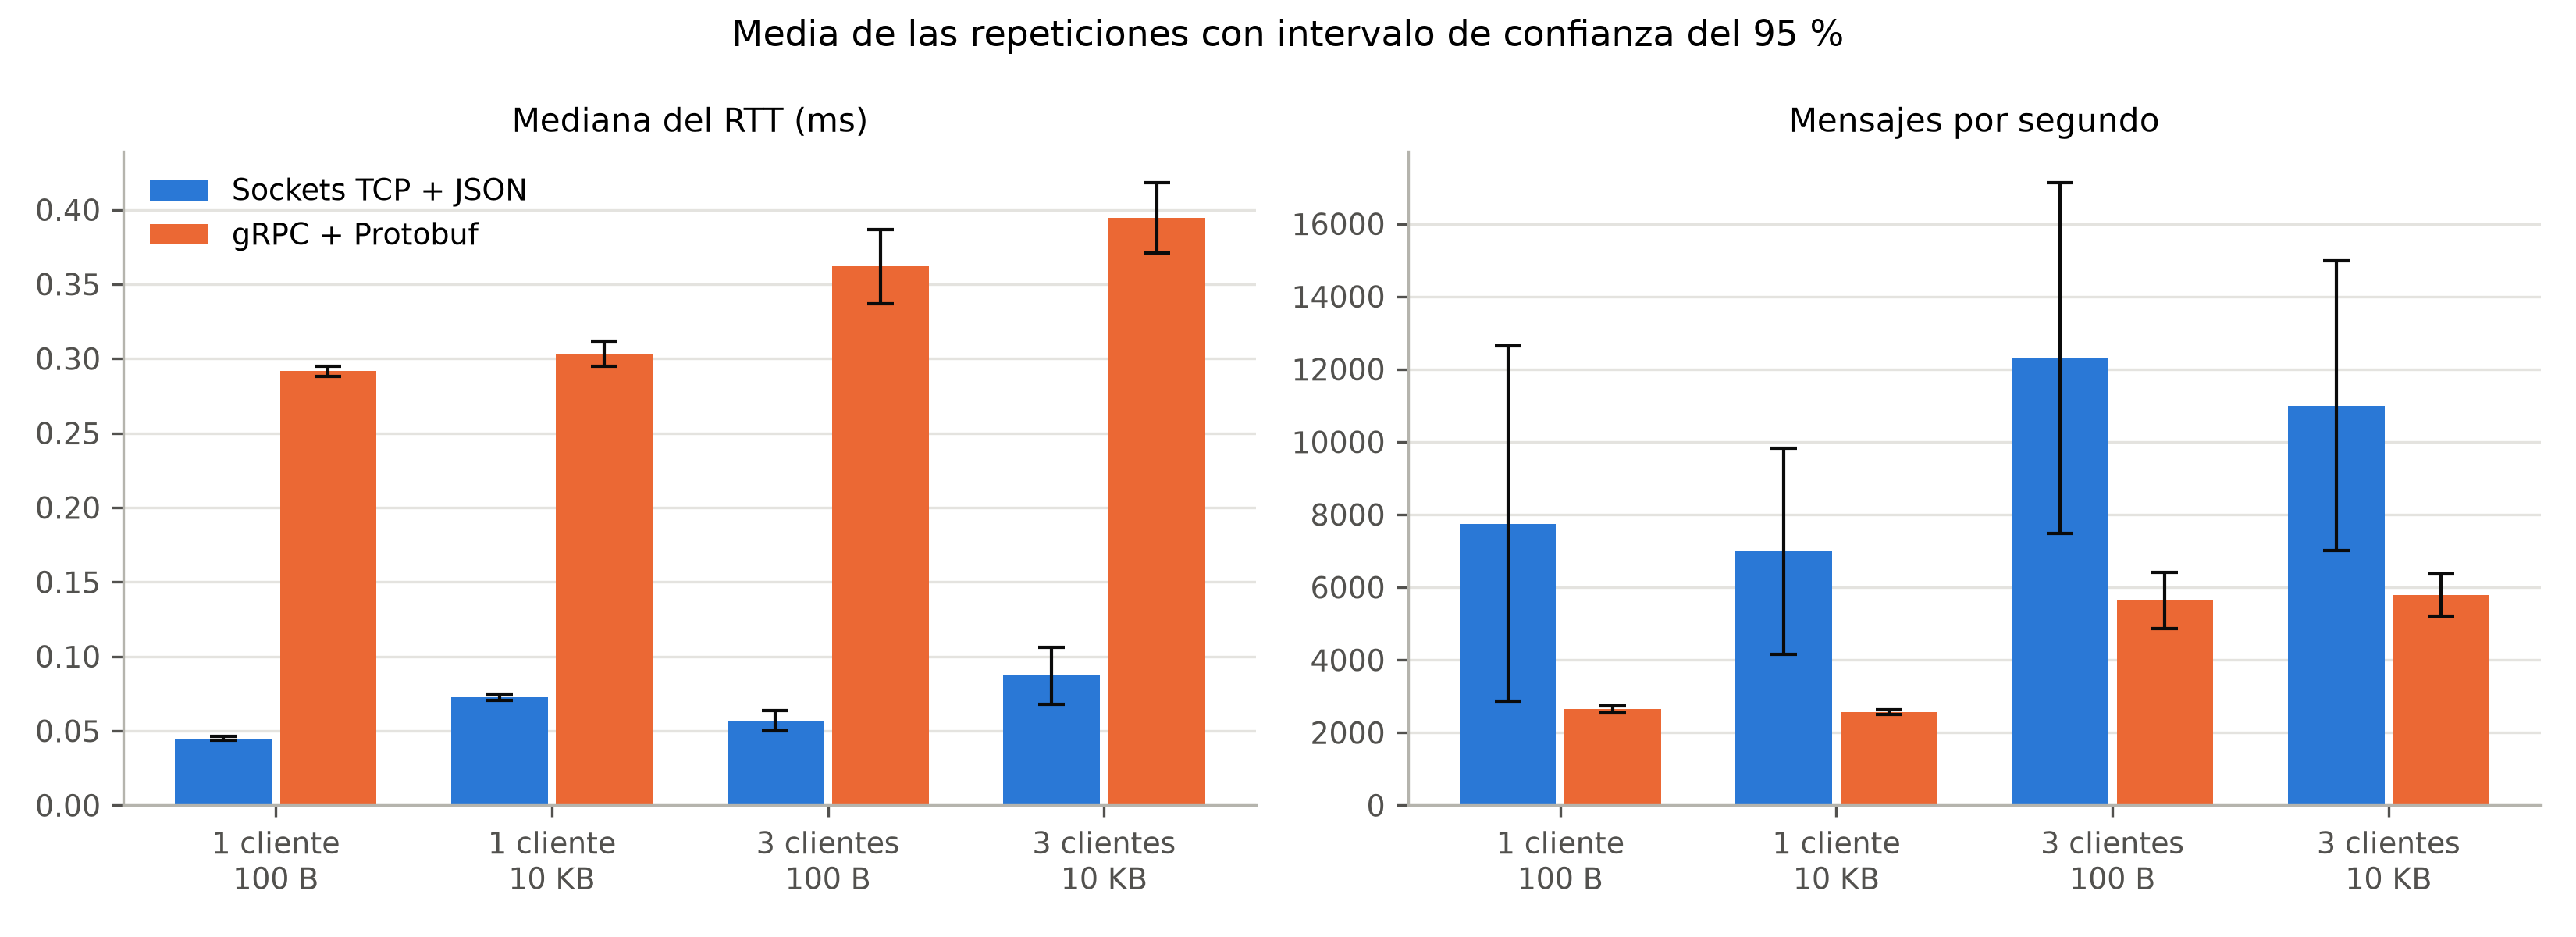
\includegraphics[width=\textwidth]{barras}
  \caption{Mediana del RTT y mensajes por segundo: media de las cinco repeticiones con intervalo de confianza del 95\,\%}
  \label{fig:barras}
\end{figure}

\subsection{Resultado de H1, H2 y H3}

\begin{table}[htbp]
  \centering
  \caption{Criterio de decisión aplicado a las hipótesis de latencia}
  \label{tab:hipotesis}
  \small
  % Generado por analysis/analizar.py. No editar a mano.
\begin{tabular}{>{\raggedright\arraybackslash}p{0.8cm} >{\raggedright\arraybackslash}p{2.6cm} >{\raggedright\arraybackslash}p{8.6cm} l}
\toprule
Hip. & Condición & Detalle & ¿Se cumple? \\
\midrule
H1 & 100 B, 1 cliente & mediana menor: sí; p95 menor: sí; más msg/s: sí & sí \\
H2 & 10 KB vs 100 B, 1 cliente & mediana menor con 10 KB: sí; cocientes 10 KB [3,97; 4,42] < cocientes 100 B [6,26; 6,85]: sí & sí \\
H3 & 100 B, 3 clientes vs 1 & mediana menor: sí; p95 menor: sí; cocientes 3 clientes [5,21; 7,49] > cocientes 1 cliente [6,26; 6,85]: no & no \\
\bottomrule
\end{tabular}

\end{table}

La Tabla~\ref{tab:hipotesis} aplica el criterio de la sección~1 a los valores de cada repetición. H1 se cumple: en la mediana, en el percentil~95 y en los mensajes por segundo, los rangos de las cinco repeticiones de los dos mecanismos no se traslapan. Incluso la peor repetición de sockets (3316 mensajes por segundo) supera a la mejor de gRPC (2737).

H2 también se cumple. Con 10~KB sockets mantiene menor mediana que gRPC, y los 25 cocientes entre las medianas de gRPC y de sockets con 10~KB (de 3,97 a 4,42) quedan todos por debajo de los 25 cocientes con 100~bytes (de 6,26 a 6,85).

H3 no se cumple. Con tres clientes, sockets tiene menor mediana y menor percentil~95 que gRPC, pero sus cocientes (de 5,21 a 7,49) se traslapan con los de un cliente. Con este criterio no se puede afirmar que la ventaja relativa de sockets haya crecido.

\subsection{Relojes de Lamport y convergencia}

En las 78 corridas se recibieron 20\,400 mensajes. En todos, el reloj de la recepción fue mayor que el del envío, y no quedó ningún envío sin su recepción. La verificación completa está en la sección de los relojes de Lamport.

\begin{table}[htbp]
  \centering
  \caption{Convergencia de los relojes de Lamport en las corridas de 20 intercambios}
  \label{tab:convergencia}
  \resizebox{\textwidth}{!}{% Generado por analysis/analizar.py desde analysis/lamport_convergencia.csv.
% No editar a mano.
\begin{tabular}{llrrrrrrr}
\toprule
Mecanismo & Nodos & Corridas & Convergen & Intercambios & Mín. (ms) & Mediana (ms) & Máx. (ms) & $>$100 ms \\
\midrule
Sockets TCP + JSON & 2 & 5 & 5 & 2 & 4,7 & 15,6 & 513,9 & 1 \\
Sockets TCP + JSON & 3 & 5 & 5 & 6 & 13,3 & 29,3 & 532,0 & 2 \\
Sockets TCP + JSON & 4 & 5 & 5 & 8 & 30,4 & 518,7 & 563,6 & 4 \\
gRPC + Protobuf & 2 & 5 & 5 & 2 & 5,6 & 5,7 & 6,3 & 0 \\
gRPC + Protobuf & 3 & 5 & 5 & 6 & 11,0 & 11,2 & 515,1 & 1 \\
gRPC + Protobuf & 4 & 5 & 5 & 8 & 11,6 & 13,0 & 21,9 & 0 \\
\bottomrule
\end{tabular}
}
\end{table}

Las 30 corridas de intercambios convergieron dentro de los 20 mensajes (Tabla~\ref{tab:convergencia}). El número de intercambios fue el mismo en todas las repeticiones de cada caso: 2 con dos nodos, 6 con tres y 8 con cuatro. Con los tiempos aparecen dos grupos. La mayoría de las corridas convergió entre 4,7 y 30,4~ms, pero 8 de las 30 tardaron más de medio segundo: 7 de sockets y 1 de gRPC. Las medianas con gRPC fueron 5,7, 11,2 y 13,0~ms para 2, 3 y 4 nodos; con sockets, 15,6, 29,3 y 518,7~ms.

Con el criterio de la sección~1, H4 no se cumple. El número de intercambios sí crece de 2 a 3 y a 4 nodos, pero no da 2, 4 y 6 como esperábamos. En el tiempo, los rangos se traslapan en los dos mecanismos; por ejemplo, una corrida de gRPC con 3 nodos tardó 515~ms, más que cualquiera de las de 4 nodos. La sección~\ref{sec:discusion-lamport} explica las dos cosas.
